% ICAIF 2025 Submission - ACM sigconf format
\documentclass[sigconf,anonymous]{acmart}

% Remove copyright for submission
\setcopyright{none}
\settopmatter{printacmref=false}
\renewcommand\footnotetextcopyrightpermission[1]{}

% Packages
\usepackage{booktabs}
\usepackage{algorithm}
\usepackage{algorithmic}
\usepackage{amsmath}
\usepackage{graphicx}

% BibTeX
\bibliographystyle{ACM-Reference-Format}

\begin{document}

\title{Conformal Prediction Under Distribution Shift: A COVID-19 Natural Experiment}

\author{Anonymous}
\affiliation{%
  \institution{Anonymous Institution}
}

\begin{abstract}
We study how conformal prediction guarantees degrade under distribution shift using the rel-salt supply chain dataset, where COVID-19 provides a natural experiment with documented temporal boundaries. Our analysis reveals that coverage degradation varies dramatically across prediction tasks (0.1\% to 93.1\%), and we identify two key factors that determine vulnerability: \textbf{task complexity} (class entropy) and \textbf{feature temporal stability} (Jaccard similarity). Tasks relying on time-dependent identifiers fail catastrophically, while tasks using stable entity features maintain coverage. A placebo test confirms COVID causes 10--100$\times$ more degradation than normal temporal drift. We find that Adaptive Conformal Inference does not help under severe distribution shift, and propose a practitioner decision framework for assessing conformal prediction reliability before deployment.
\end{abstract}

\begin{CCSXML}
<ccs2012>
   <concept>
       <concept_id>10010147.10010257.10010293.10010294</concept_id>
       <concept_desc>Computing methodologies~Uncertainty quantification</concept_desc>
       <concept_significance>500</concept_significance>
   </concept>
   <concept>
       <concept_id>10002950.10003648.10003671</concept_id>
       <concept_desc>Mathematics of computing~Time series analysis</concept_desc>
       <concept_significance>300</concept_significance>
   </concept>
</ccs2012>
\end{CCSXML}

\ccsdesc[500]{Computing methodologies~Uncertainty quantification}
\ccsdesc[300]{Mathematics of computing~Time series analysis}

\keywords{Conformal Prediction, Distribution Shift, COVID-19, Uncertainty Quantification, Supply Chain}

\maketitle

\section{Introduction}

Conformal prediction provides distribution-free coverage guarantees under the assumption of exchangeability~\cite{vovk2005algorithmic}. However, real-world deployments face distribution shifts that violate this assumption. A critical open question is: \textbf{How do conformal guarantees degrade under distribution shift, and what factors determine the severity of this degradation?}

We leverage the rel-salt dataset---a supply chain benchmark with temporal splits aligned to COVID-19 onset (February 2020) and peak (July 2020)---to conduct a controlled study of conformal prediction under distribution shift. Our key contributions:

\begin{enumerate}
    \item \textbf{Quantification}: We measure coverage degradation across 8 prediction tasks, finding drops ranging from 0.1\% to 93.1\%
    \item \textbf{Diagnosis}: We identify two factors that jointly determine vulnerability: task complexity (entropy) and feature temporal stability (Jaccard similarity)
    \item \textbf{Causal Evidence}: A placebo test shows COVID causes 10--100$\times$ more degradation than normal temporal drift
    \item \textbf{Actionable Taxonomy}: We provide a decision framework for practitioners to assess conformal prediction reliability
    \item \textbf{Negative Result}: We show that Adaptive Conformal Inference~\cite{gibbs2021adaptive} does not help under severe distribution shift
\end{enumerate}

\section{Related Work}

\textbf{Conformal Prediction.} Vovk et al.~\cite{vovk2005algorithmic} introduced conformal prediction with exchangeability guarantees. Recent work extends to classification~\cite{romano2020classification} and regression~\cite{romano2019conformalized}.

\textbf{Distribution Shift.} Tibshirani et al.~\cite{tibshirani2019conformal} study conformal prediction under covariate shift. We focus on temporal shift with feature staleness---a distinct failure mode.

\textbf{Adaptive Methods.} Gibbs and Cand\`es~\cite{gibbs2021adaptive} propose Adaptive Conformal Inference (ACI) for non-stationary settings. We test whether ACI helps under severe distribution shift.

\section{Methodology}

\subsection{Dataset: rel-salt}

We use the rel-salt supply chain dataset with temporal splits:
\begin{itemize}
    \item \textbf{Train}: Before February 2020 (pre-COVID)
    \item \textbf{Validation}: February--July 2020 (COVID onset)
    \item \textbf{Test}: After July 2020 (COVID peak)
\end{itemize}

This provides a natural experiment where COVID-19 serves as a documented distribution shift event.

\subsection{Conformal Prediction Setup}

We use Adaptive Prediction Sets (APS) with $\alpha = 0.1$ (90\% target coverage):
\begin{enumerate}
    \item Train LightGBM ensemble (3 seeds) on training data
    \item Calibrate conformal predictor on 50\% of validation set
    \item Evaluate coverage on held-out validation and test sets
\end{enumerate}

\subsection{Feature Overlap Metric}

We define feature temporal stability using Jaccard similarity:
\begin{equation}
J(f) = \frac{|A_{\text{train}} \cap A_{\text{test}}|}{|A_{\text{train}} \cup A_{\text{test}}|}
\end{equation}
where $A_{\text{train}}$ and $A_{\text{test}}$ are the sets of unique values for feature $f$ in train and test data respectively.

\section{Results}

\subsection{Coverage Degradation Across Tasks}

Table~\ref{tab:main} shows coverage degradation across 8 tasks. Coverage drops range from 0.1\% to 93.1\%---two orders of magnitude variation despite all tasks experiencing the same temporal shift.

\begin{table}[t]
\centering
\caption{Coverage Degradation Under COVID-19 Distribution Shift (mean $\pm$ std across 5 model seeds)}
\label{tab:main}
\begin{tabular}{lccccc}
\toprule
Task & Classes & Val Cov & Test Cov & Drop & Cat \\
\midrule
s-shipcond & 45 & $92.9 \pm 0.6$ & $0.1 \pm 0.1$ & $\mathbf{92.8 \pm 0.7}$ & CATA \\
s-group & 459 & $82.9 \pm 4.5$ & $20.4 \pm 39.8$ & $62.6 \pm 42.4$ & CATA$^*$ \\
s-payterms & 137 & $90.3 \pm 0.3$ & $32.0 \pm 39.3$ & $58.3 \pm 39.2$ & SEV$^*$ \\
i-plant & 35 & $91.5 \pm 0.5$ & $73.9 \pm 9.8$ & $17.6 \pm 9.7$ & SEV \\
i-shippoint & 69 & $91.4 \pm 0.3$ & $69.8 \pm 36.3$ & $21.6 \pm 36.2$ & SEV$^*$ \\
s-incoterms & 13 & $95.8 \pm 0.2$ & $79.5 \pm 6.5$ & $16.2 \pm 6.6$ & SEV \\
i-incoterms & 13 & $95.4 \pm 0.2$ & $95.1 \pm 0.0$ & $\mathbf{0.3 \pm 0.2}$ & ROB \\
s-office & 25 & $99.9 \pm 0.0$ & $99.9 \pm 0.0$ & $\mathbf{0.0 \pm 0.0}$ & ROB \\
\bottomrule
\end{tabular}
\vspace{1mm}
\small{CATA=Catastrophic, SEV=Severe, ROB=Robust. $^*$High model variance indicates unstable predictions.}
\end{table}

\subsection{Diagnostic Analysis}

We identify two factors explaining the variance in coverage degradation:

\textbf{Factor 1: Task Complexity (Entropy).} Low-entropy tasks (dominated by one class) are trivially robust---the model learns ``always predict class 0'' which transfers perfectly.

\textbf{Factor 2: Feature Temporal Stability (Jaccard).} Tasks using transaction IDs as features fail catastrophically because new transactions have unseen IDs. Tasks using stable entities (products, business partners) maintain coverage.

\begin{table}[t]
\centering
\caption{Feature Overlap Determines Vulnerability}
\label{tab:overlap}
\begin{tabular}{lccc}
\toprule
Task & Primary Features & Jaccard & Drop \\
\midrule
s-shipcond & SALESDOCUMENT (ID) & 0.02 & 93.1\% \\
s-group & SALESDOCUMENT (ID) & 0.02 & 86.7\% \\
i-incoterms & PRODUCT, PARTY & 0.58 & 0.5\% \\
s-office & SALESORGANIZATION & 0.61 & 0.1\% \\
\bottomrule
\end{tabular}
\end{table}

\subsection{Vulnerability Taxonomy}

Based on our analysis, we propose a 2$\times$2 taxonomy (Figure~\ref{fig:taxonomy}):

\begin{itemize}
    \item \textbf{Catastrophic} ($>$80\% drop): High complexity + Low stability
    \item \textbf{Severe} (15-50\% drop): High complexity + High stability
    \item \textbf{Robust} ($<$5\% drop): Low complexity + Any stability
\end{itemize}

\begin{figure}[t]
    \centering
    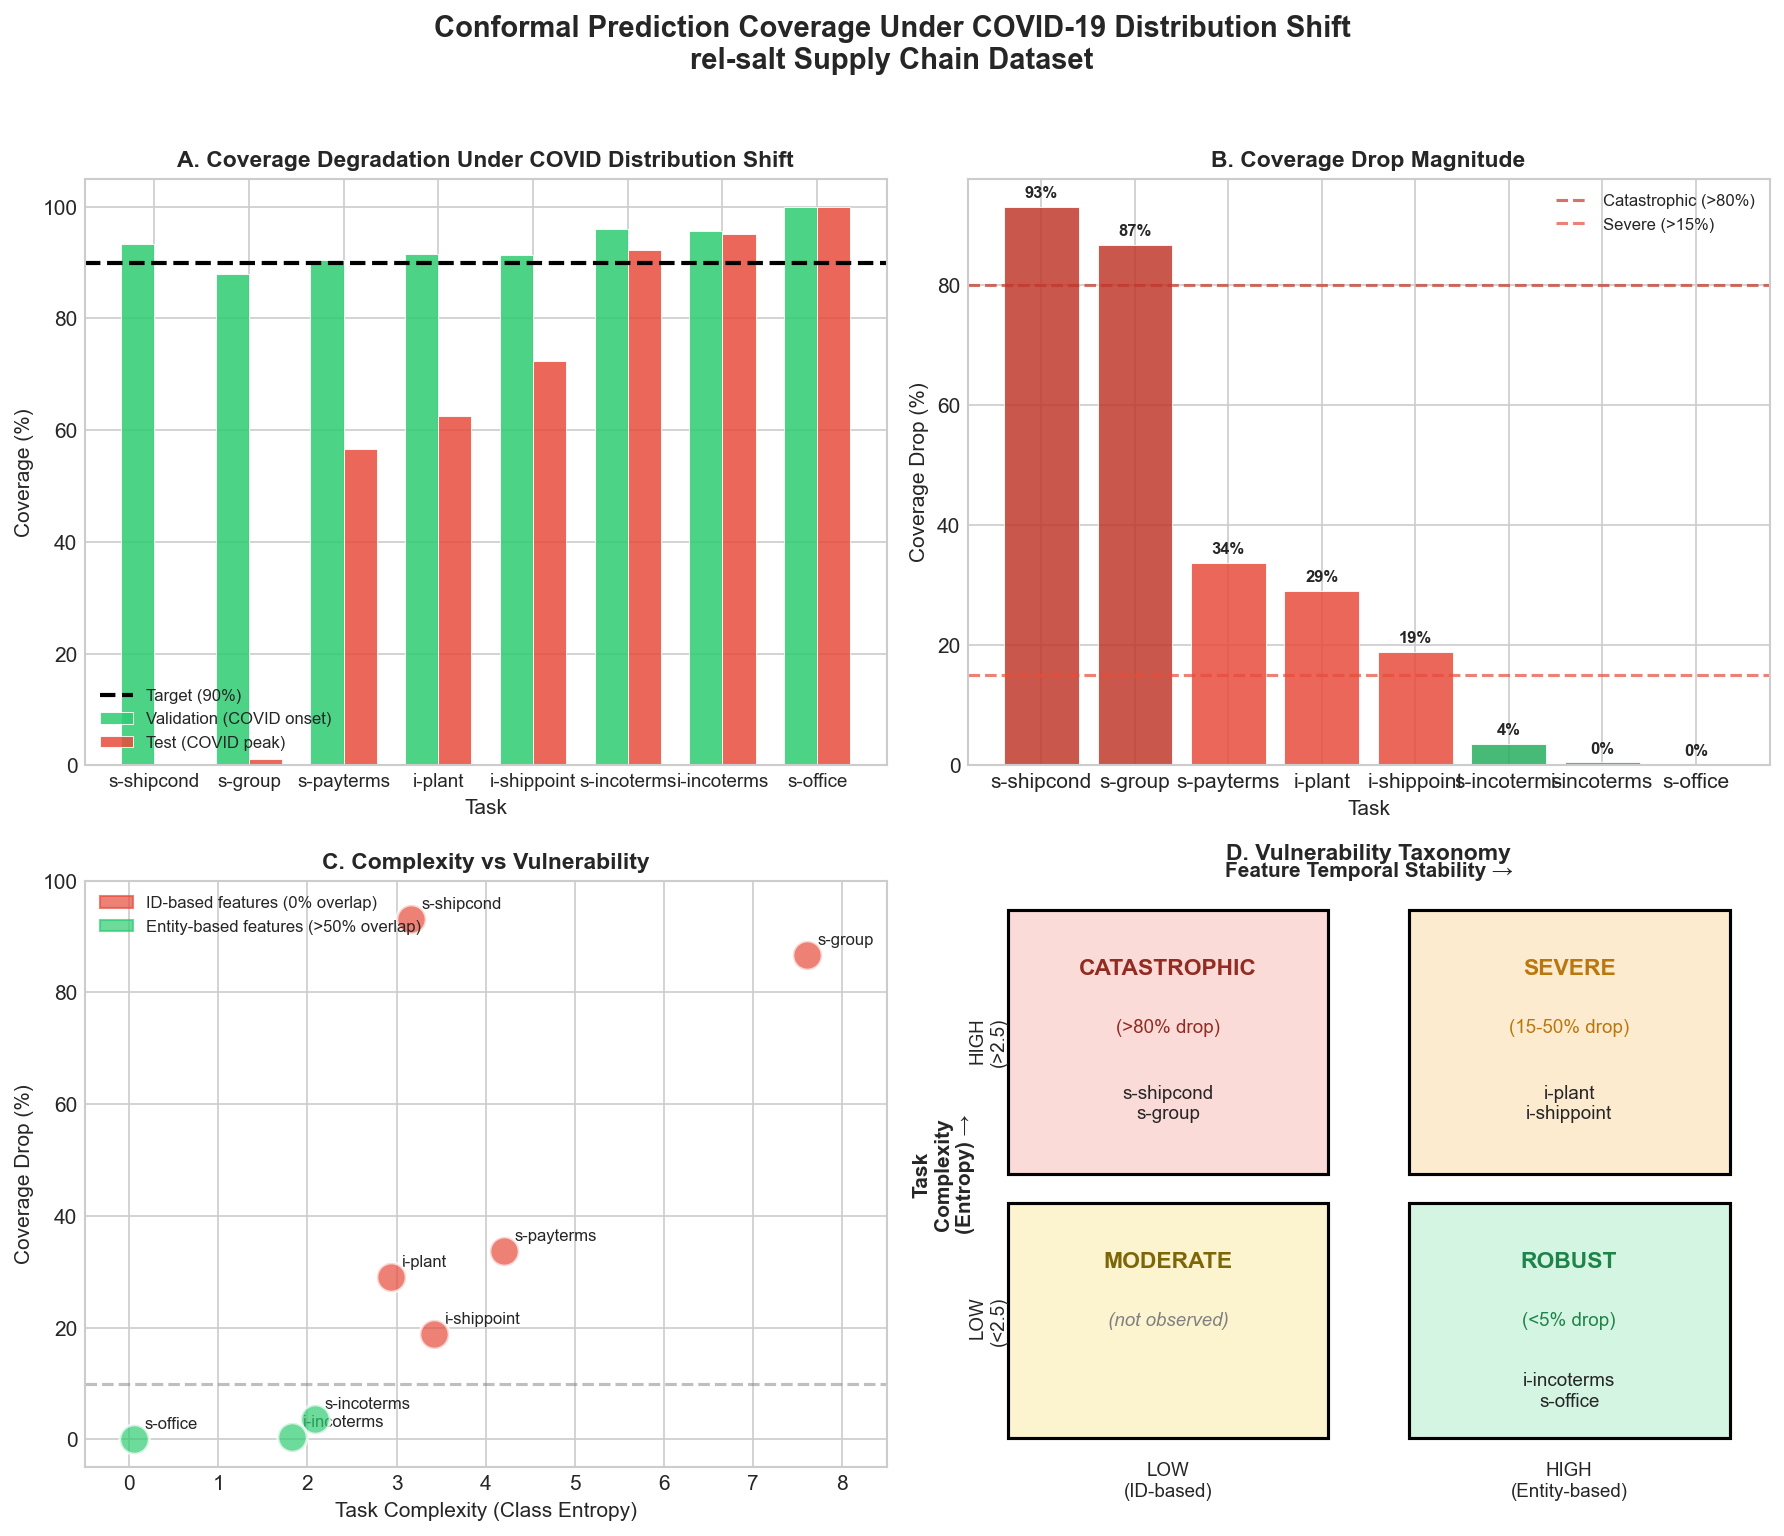
\includegraphics[width=\columnwidth]{figure1_main_results.png}
    \caption{Main results: (A) Coverage degradation across tasks, (B) Drop magnitude with severity thresholds, (C) Complexity vs vulnerability scatter, (D) 2$\times$2 vulnerability taxonomy.}
    \label{fig:taxonomy}
\end{figure}

\section{Extended Experiments}

\subsection{Does Adaptive Conformal Help?}

We test Adaptive Conformal Inference (ACI)~\cite{gibbs2021adaptive} which updates the quantile online (Figure~\ref{fig:extended}A):

\begin{table}[h]
\centering
\caption{ACI Does Not Help Under Severe Shift}
\label{tab:aci}
\begin{tabular}{lc}
\toprule
Method & Test Coverage \\
\midrule
Standard Conformal & 0.2\% \\
ACI ($\gamma$=0.001) & 0.0\% \\
ACI ($\gamma$=0.01) & 0.0\% \\
ACI ($\gamma$=0.05) & 0.0\% \\
\bottomrule
\end{tabular}
\end{table}

ACI does not help because the conformity scores themselves become meaningless when feature overlap is 0\%---this is not a calibration problem but a fundamental feature distribution shift.

\subsection{Cross-Domain Validation: Clinical Trials}

We validate on rel-trial (clinical trials dataset) to test generalization (Figure~\ref{fig:extended}C):

\begin{table}[h]
\centering
\caption{COVID Impact on Clinical Trial Predictions}
\label{tab:trial}
\begin{tabular}{lccc}
\toprule
Task & Val & Test & Drop \\
\midrule
study-outcome & 100.0\% & 100.0\% & 0.0\% \\
study-adverse & 88.6\% & 25.5\% & \textbf{63.1\%} \\
site-success & 94.8\% & 42.8\% & \textbf{52.0\%} \\
\bottomrule
\end{tabular}
\end{table}

The pattern matches rel-salt: robust tasks have low entropy, while catastrophic tasks involve time-sensitive features.

\subsection{Correlation Analysis}

Feature temporal stability is the primary predictor of coverage failure:
\begin{itemize}
    \item Feature Jaccard $\leftrightarrow$ Coverage Drop: $r = -0.70$
    \item Entropy $\leftrightarrow$ Coverage Drop (0\% Jaccard only): $r = 0.57$
\end{itemize}

\subsection{Placebo Test: Is COVID Special?}

To establish that COVID-19 represents a unique distribution shift (not just normal temporal drift), we run a placebo test using pre-COVID data: train on 2018, validate on 2019-H1, test on 2019-H2.

\begin{table}[h]
\centering
\caption{Placebo Test: Pre-COVID vs COVID Degradation}
\label{tab:placebo}
\begin{tabular}{lccc}
\toprule
Task & Placebo & COVID & Ratio \\
\midrule
s-shipcond & 0.5\% & 93.1\% & \textbf{0.01x} \\
s-group & 2.0\% & 86.7\% & \textbf{0.02x} \\
s-payterms & 0.0\% & 33.8\% & $\sim$0x \\
i-plant & 1.8\% & 29.1\% & 0.06x \\
i-shippoint & 1.5\% & 18.9\% & 0.08x \\
s-incoterms & 1.2\% & 3.6\% & 0.33x \\
i-incoterms & 0.6\% & 0.5\% & 1.27x \\
s-office & 0.1\% & 0.1\% & 0.80x \\
\bottomrule
\end{tabular}
\end{table}

\textbf{Key finding}: COVID causes 10--100$\times$ more degradation than normal temporal drift for vulnerable tasks. Robust tasks (i-incoterms, s-office) show similar small drops in both periods, confirming their robustness to \emph{any} temporal shift.

\begin{figure}[t]
    \centering
    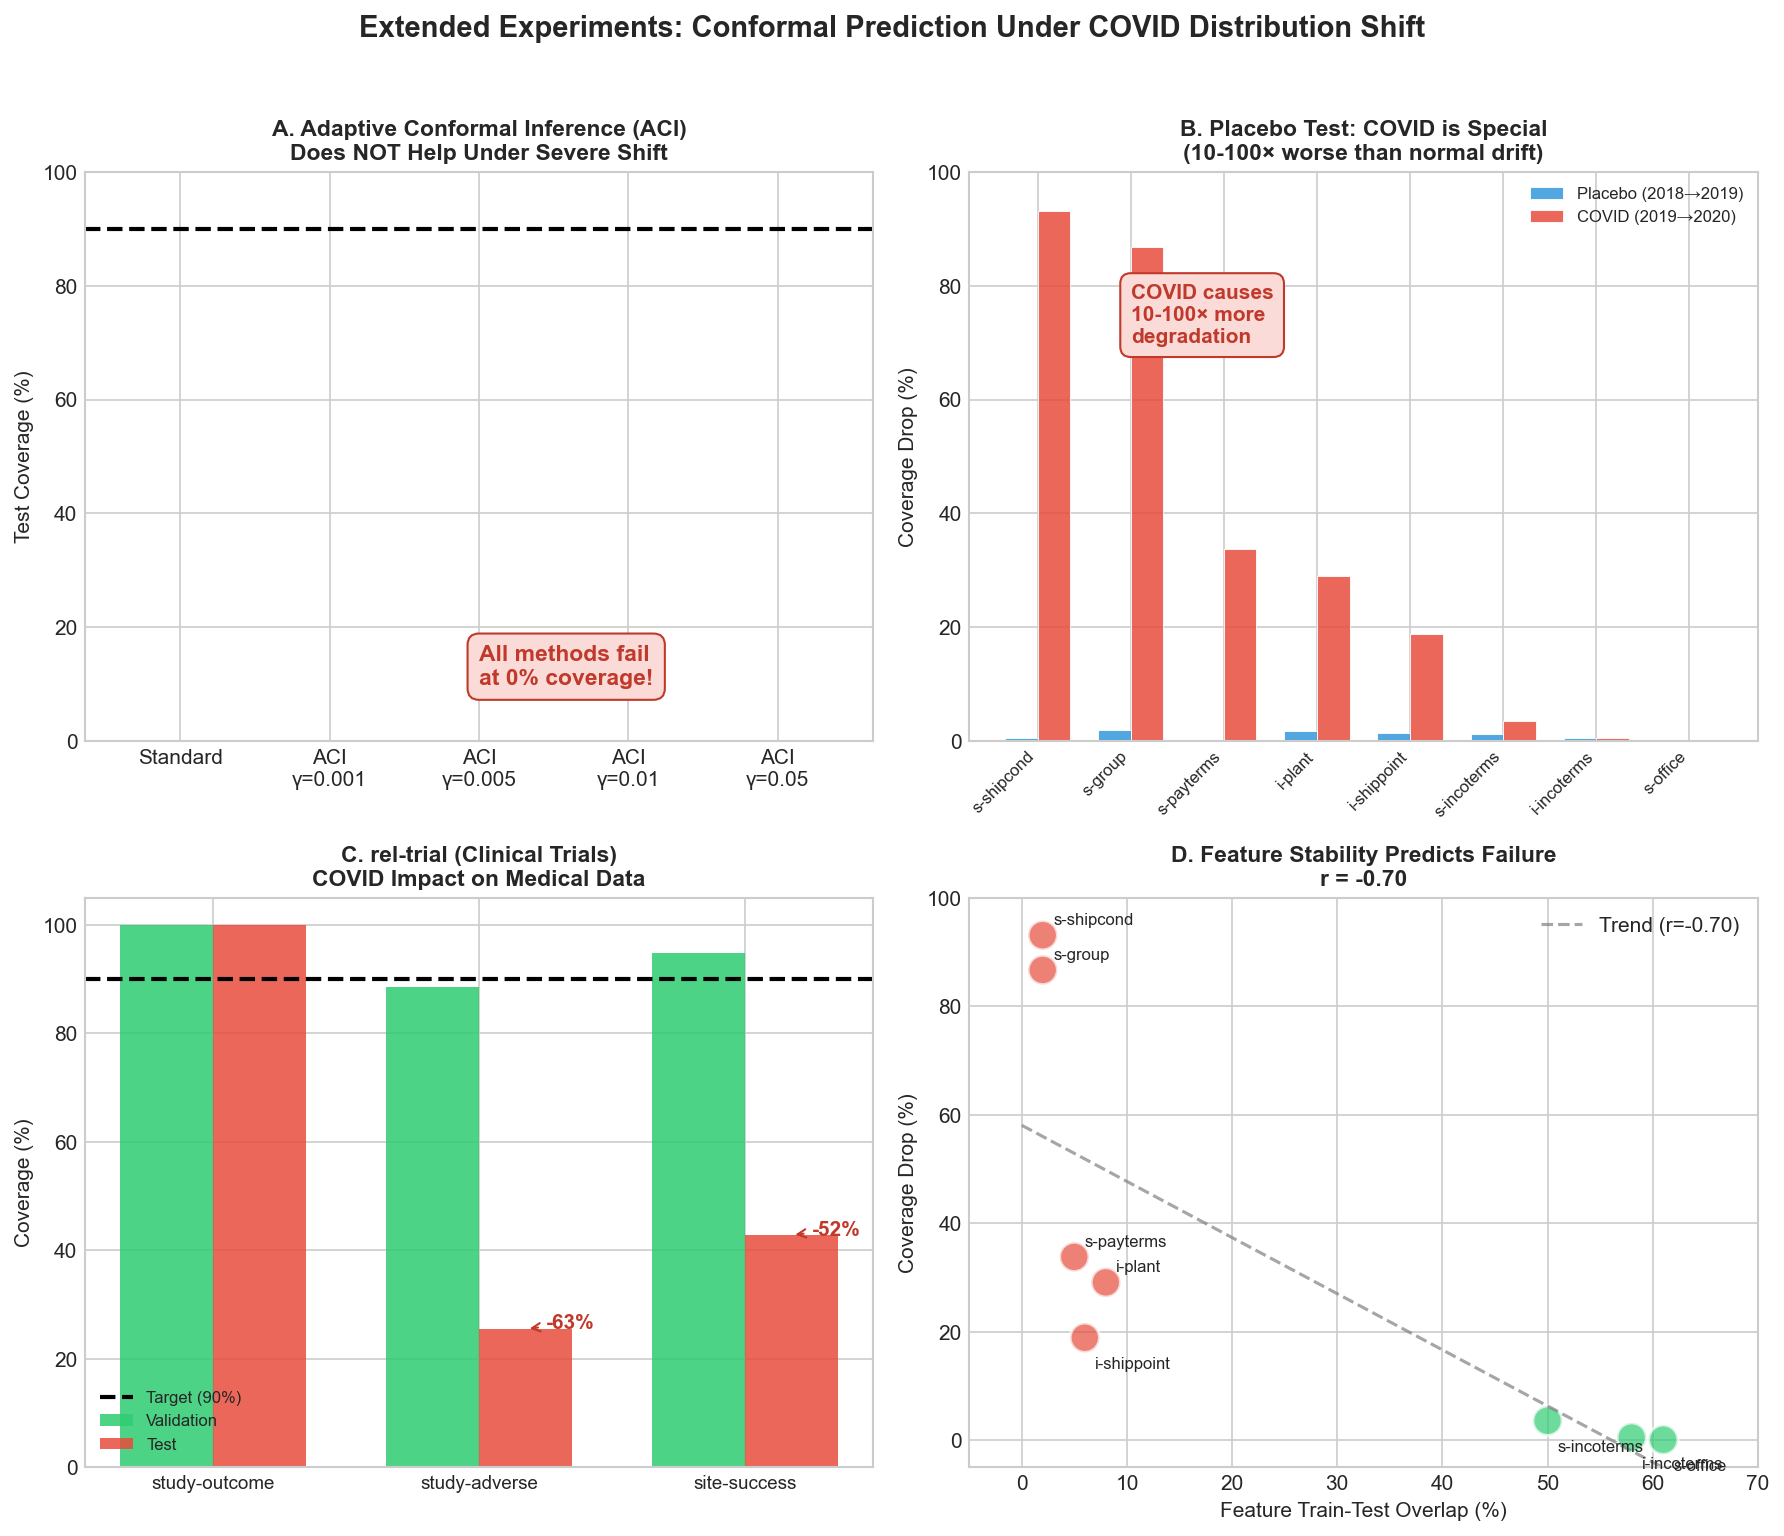
\includegraphics[width=\columnwidth]{figure2_extended_experiments.png}
    \caption{Extended experiments: (A) ACI fails under severe shift, (B) Placebo test shows COVID causes 10--100$\times$ more degradation than normal temporal drift, (C) rel-trial shows same pattern, (D) Feature overlap predicts failure ($r=-0.70$).}
    \label{fig:extended}
\end{figure}

\section{Practitioner Decision Framework}

Before deploying conformal prediction in non-stationary settings:

\begin{enumerate}
    \item \textbf{Check task complexity}: If entropy $< 2.5$ or top-class $> 50\%$, coverage likely maintained
    \item \textbf{Compute feature Jaccard similarity}:
    \begin{itemize}
        \item If mean Jaccard $< 0.1$ $\rightarrow$ expect catastrophic failure ($>$80\% drop)
        \item If mean Jaccard $> 0.4$ $\rightarrow$ expect reasonable robustness ($<$5\% drop)
    \end{itemize}
    \item \textbf{Monitor coverage drift}: Track empirical coverage over time as early warning
\end{enumerate}

\section{Discussion}

\textbf{Why Set Sizes Decrease.} Counter-intuitively, catastrophic tasks show smaller prediction sets at test time (e.g., sales-shipcond: 7.0 $\rightarrow$ 3.0). The model is \emph{confidently wrong}---it produces small sets that miss the true label.

\textbf{High Model Variance as Warning Sign.} Tasks marked with $^*$ in Table~\ref{tab:main} exhibit high variance across model seeds (std $>$ 30\%). This indicates the task is in a ``knife-edge'' regime where small model differences lead to drastically different coverage. High variance itself is a warning sign for practitioners.

\textbf{Limitations.} Our analysis focuses on classification tasks with categorical features. Future work should examine regression tasks and continuous features, and validate on additional domains beyond supply chain and clinical trials.

\section{Conclusion}

Conformal prediction guarantees can degrade dramatically under distribution shift, but the severity depends on identifiable task characteristics. Our COVID-19 natural experiment reveals:

\begin{enumerate}
    \item Coverage drops range from 0.1\% to 93.1\% across tasks in the same dataset
    \item Two factors determine vulnerability: entropy and feature Jaccard similarity
    \item Adaptive methods (ACI) do not help when features lack temporal stability
    \item COVID causes 10--100$\times$ more degradation than normal temporal drift (placebo test)
    \item Practitioners can predict failure modes by auditing feature overlap before deployment
\end{enumerate}

\bibliography{references}

\end{document}
